% file: katomicity-trace-not12atomic.tex

\documentclass[tikz]{standalone}
\usetikzlibrary{positioning, arrows.meta, calc, fit, shapes}

% command for interval
\newcommand{\itv}[4]{ % #1: start point; #2: end point; #3: operation name; #4: color
  \coordinate (start #3) at #1;	% start point
  \coordinate (end #3) at #2;	% end point

  \draw[ultra thick, #4, |-|] (start #3) -- (end #3) % draw the interval
  	node[pos = 0.5, above = 1mm, font = \Large, text=black] (#3) {$#3$}; % attach the operation name
}

\begin{document}
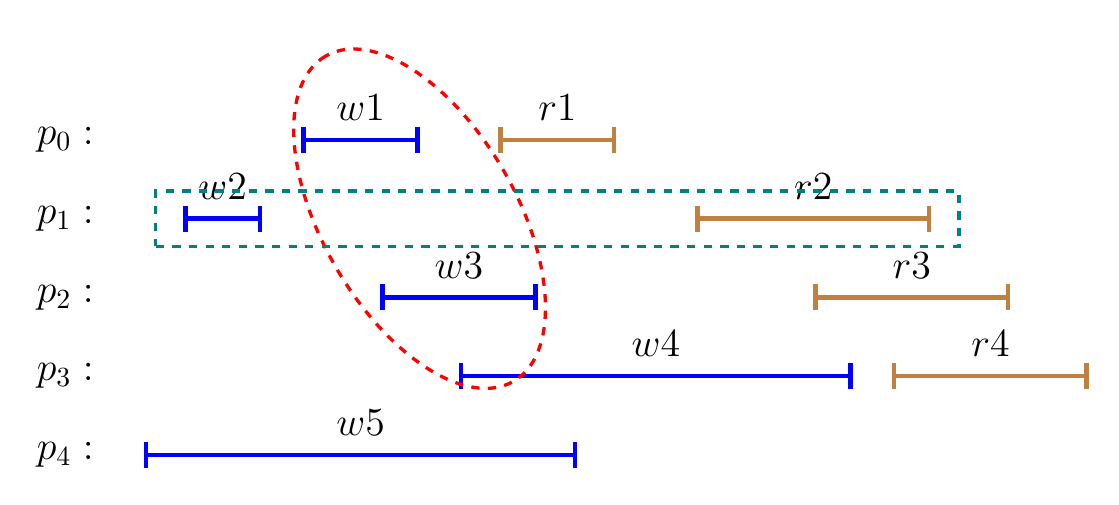
\begin{tikzpicture}[txt/.style = {font = \Large}]
  \itv{(0,0)}{(5.5,0)}{w5}{blue}
  \itv{(0.5,3)}{(1.5,3)}{w2}{blue}
  \itv{(2,4)}{(3.5,4)}{w1}{blue}
  \itv{(3,2)}{(5,2)}{w3}{blue}
  \itv{(4,1)}{(9,1)}{w4}{blue}
  \itv{(4.5,4)}{(6,4)}{r1}{brown}
  \itv{(7,3)}{(10,3)}{r2}{brown}
  \itv{(8.5,2)}{(11,2)}{r3}{brown}
  \itv{(9.5,1)}{(12,1)}{r4}{brown}

  \node (p0) [txt] at (-1, 4) {$p_0:$};
  \node (p1) [txt] at (-1, 3) {$p_1:$};
  \node (p2) [txt] at (-1, 2) {$p_2:$};
  \node (p3) [txt] at (-1, 1) {$p_3:$};
  \node (p4) [txt] at (-1, 0) {$p_4:$};

  \node () [draw, ellipse, very thick, red, dashed, inner sep = 2pt, rotate fit = 120, fit = (start w1) (end w3)] {};
  \node () [draw, rectangle, very thick, teal, dashed, inner sep = 10pt, fit = (start w2) (end r2)] {};
\end{tikzpicture}
\end{document}
